\documentclass{article}
\usepackage{graphicx}
\usepackage{changes}
\usepackage{lipsum}% <- For dummy text
\usepackage{subcaption}
\usepackage{natbib}
\usepackage{setspace}
\usepackage{tablefootnote}
\usepackage{amsmath}% http://ctan.org/pkg/amsmath
\usepackage{kbordermatrix}% http://www.hss.caltech.edu/~kcb/TeX/kbordermatrix.sty
\captionsetup{compatibility=false}
\definechangesauthor[name={Per cusse}, color=orange]{per}

     
\begin{document}
\title{The effect of Influenza receptor binding on antigenic drift}
\author{Hsiang-Yu Yuan}
\maketitle

\bibliographystyle{plainnat}
\nocite{*}

\doublespacing
\begin{abstract}

Influenza viruses circulating in humans are known to undergo rapid antigenic evolution. Significant work remains, however, in understanding the selective drivers of these evolutionary dynamics. Influenza’s antigenic drift is commonly thought to arise from selection of immunity acting directly on drift variants, resulting in the increase of susceptible hosts to them. 

A recent study by Hensley and coauthors proposed that influenza’s antigenic drift could be driven from alternative changes of cellular receptor binding. However, the evolution of the receptor binding and their effects on the course of infection in the population remains poorly understood.  

Here, using influenza netcharge as markers for binding avidity, we demonstrate the binding avidity significantly associated by hosts ages, consistent to the immune evasion mechanism previously observed in Ferret. However, at the population level, phylogenetic analysis of viral sequences show that receptor binding avidity appears to be under stabilizing selection. We therefore propose that the binding avidity changes within individuals towards either high or low binding avidity is a case of ‘short-sighted’ evolution that might decrease a virus’s potential transmissibility at the level of the population.

When most drift variants are weak, binding avidity changes would drive the drift. If the large effect drift variants occur, the effect of binding avidity on the drift diminished. A strong antigenic mutant accompanied with binding avidity change would lead the optimum selection fitness.   

\end{abstract}






\section{Materials and Methods}

\subsection{Virus infection model}

The host immunity would be boosted during an infection and protects the host from being infected again if contact with the similar viruses. Once the host is contacted with the same antigenic strain, the probability of the virus to survive in the presence of the host immunity is defined as
\begin{equation}
    \label{simple_equation}
    f(V_{i}) = [1-e^{-p(V_{i}+1)}]^{rk} \\
\end{equation}

where $e^{-p(V_{i}+1)}$ is the proportion that viruses cleared by antibodies and $D$ is the antigenic distance between the host immunity and the viruses that boost the immunity. When the infection history $H$ is considered, the probability of viruses survival becomes the joint survival probability among all cross-reactive immunity boosted by each strains

\begin{equation}
    \label{simple_equation}
    \begin{split}
    f(H,V_{i}) &= \prod_{j=1}^{k} [1-e^{-p(V_{i}+1)}]^{(rk-\delta_{ji})} \\
    \end{split}
\end{equation}
\begin{equation}
\space = [1-e^{-p(V_{i}+1)}]^{\Sigma_{j=1}^{k}(rk-\delta_{ji})} \\
\end{equation}

\begin{equation}
    \label{simple_equation}
    \begin{split}
    f(H,V_{i}) &= \prod_{j=1}^{k} [1-e^{-p(V_{i}+1)}]^{\frac{1}{D+\alpha_{i}}} \
    \end{split}
\end{equation}
\begin{equation}
\space = [1-e^{-p(V_{i}+1)}]^{\frac{1}{\lambda}} \\
\end{equation}
\begin{equation}
\lambda = \frac{1}{\Sigma{\frac{1}{D_{i}+\alpha_{i}}}} \\
\end{equation}


(Note: I will still prefer to use eq4, because we can project the immunity onto antigenic map)

where $\delta_{ji}$ is the antigenic distance between the the previous infecting strain $j$ and the challenging strain $i$.

In order to evaluate the evolutionary dynamics of binding avidity, we made a simplified framework with certain assumptions. First, we consider individual viruses change on their viral receptor binding but have no individual differences on antigenicity. We assume a constant immune boosting rate. Each time when infection occurs, the immune boosting occurs which create the protection effect as antigenic distance D. We also made an assumption here that the changes of antigenicity of viruses between the time of two consecutive infection is constant. Therefore, the antigenic distance between strain $j$ and $i$ becomes

\begin{equation}
 \delta_{ji} = \delta\cdot (k+1-j) \\
\end{equation}

The probability of within host virus infection per each virus becomes the product of virus survival and the cost of binding avidity (\citep{Yuan2013}). 

\begin{equation}
  \phi(H_{k},V_{i}) = [1-e^{-p(V_{i}+1)}]^{\Sigma_{j=1}^{k}\frac{1}{D+\alpha_{ji}}} \cdot e^{-aV^{b}}
%   \Lambda = \frac{1}{\Sigma{\frac{1}{D_{i}+\alpha_{i}}}} 
%   f(k,V_{i}) = [1-e^{-p(V_{i}+1)}]^{rk} \\
\end{equation} 






The probability of viral infection is (\citep{Keeling2008})
\begin{equation}
\rho=1-(\frac{1}{R_{in}})^{-v}
=1-(\frac{1}{n \cdot \phi(H_{k},V_{i})})^{-v}
\end{equation}
where we define $R_{in}$ is within host reproductive number as the product the probability of within host virus infection and the number of offspring $n$ during replication for each virus, and $v$ is the number of viruses initially transmitted.   
 
\begin{figure}[h!]
        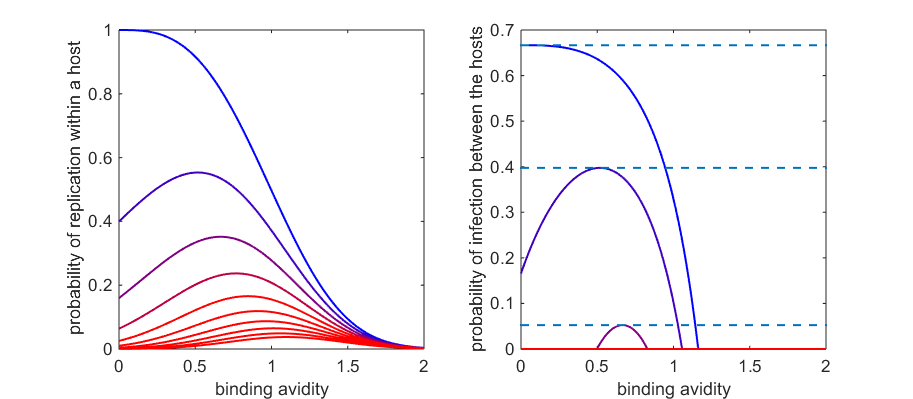
\includegraphics[width=1.2\textwidth,natwidth=8,natheight=10]{figure1.png}
        \caption{Left, the probability of virus infection within a host (eq.5). right, the probability of viral infection between the hosts (eq.6). Dashed line, infection probability without differential selection by binding avidity. }
\end{figure}

Although the virus still can replication when immunity goes stronger, the probability of viral infection quickly goes to 0 after three infections under our parameters setting, which is consistent to pandemic flu or during a single season outbreak where no significant antigenic drift was observed.
 
 
\subsection{Disease transmission simulation}
Tao-leap algorithm is used to perform disease transmission under different evolutionary scenarios. Drift Mutants generate stochastically according to the total binding avidity change in a host (mutation occurs at which day during the infectious period). The methods of disease transmission model will be written later.


Specific testing we would like to perform is: \\
Testing shortsight evolution (with constant drift, don't consider the antigenic drift driven by the binding avidity feedback):\\
1. Shortsight evolution occurs when differential selection occurs \\
2. When there is no differential selection (Figure1, right dashed line.), the effect of shortsight evolution is weaker \\
3. When a single drift variant occurs, a strong antigenic mutant temporarily decrease antigenic drift driven by binding avidity (per virus)  \\
4. Now we consider the antigenic drift driven by the binding avidity feedback: A strong antigenic mutant temporarily decrease antigenic drift driven by binding avidity(per virus)  \\


Assumption: antigenic change by binding avidity change as side effect can't be too large other wise, immune host won't be immune. Otherwise, there is no way to compare. 

\bibliography{mybinding}                
\end{document}
